\chapter[Embasamento Teórico]{Embasamento Teórico}
\label{ch:cap2}
O \textit{Power Monitor} surgiu da necessidade da conscientização do gasto energético e da melhor compreensão da conta de luz. Baseado nesse conceito,
foram desenvolvido um \textit{software} que permitirá uma fácil comunicação com qualquer equipamento construído que tenha a finalidade de monitorar a energia elétrica e um \textit{hardware} para demonstração
da comunicação entre ambos.
O sistema traz uma forma mais fácil e próxima do consumidor final de se quantificar a energia elétrica consumido em um estabelecimento. No lugar do Quilowatt-hora, medida que é usada atualmente,
o \textit{software} propõe mensurar o gasto energético em reais (R\$), trazendo a realidade do consumo mensal para mais próximo de cada brasileiro.

Esse capítulo trará os conceitos essenciais para o entendimento do trabalho, descrevendo todas as tecnologias utilizadas no desenvolvimento 
do \textit{software} como do \textit{hardware}.

\section[\textit{Ferramentas e linguagens}]{\textit{Ferramentas e linguagens}}\label{ferramenta-linguagem}
No decorrer do desenvolvimento do \textit{software} fez-se uso de algumas tecnologias e linguagens de programação que serão descrita no decorrer
dessa seção.
\subsection[\textit{Node.js}]{\textit{Node.js}}\label{node}
Node.js é um interpretador do código JavaScript (\autoref{js}), com o foco do uso da linguagem do lado do cliente para servidores. Com um objetivo simples
que é ajudar desenvolvedores na criação de aplicações de alta escalabilidade, com códigos capazes de administrar e manipulazar várias conexões simultaneamente
em um único servidor. O \textit{Node.js} é baseado na \textit{runtime} V8 \textit{JavaScript Engine}. Foi desenvolvido por Ryan Danhl em 2009, e o seu desenvolvimento
é mantido pela fundação \textit{Node.js} e \textit{Linux Foundation}. 
\subsection[\textit{JavaScript}]{\textit{JavaScript}}\label{js}
JavaScript é uma linguagem de programação interpretada de alto nível, juntamente com HTML e CSS é uma das linguagens mais utilizadads no mundo \textit{web}.
Após o uso da linguagem as páginas \textit{web} começaram a ter uma maior interatividade com o usuário. A grande maioria dos \textit{browsers} tem um
mecanismo de compilação dedicado para o JavaScript. Por ser uma linguagem multi-paradigma o JavaScript suporta paradigmas funcionais, orientados a eventos 
e até mesmo paradigmas de orientação a objeto.
Inicialmente era usada apenas no lado do cliente em \textit{web browsers}, mas atualmente está presente em vários outros tipos de \textit{softwares} incluindo
servidores - como já foi discutido na \autoref{node} - \textit{databases} e até sistemas \textit{desktop} como os leitores de PDF, programas de música e recentemente
vem ganhando espaço no desenvolvimento de aplicativos para celular.

\subsection[\textit{WebSocket}]{\textit{WebSocket}}\label{websocket}
A ideia da tecnologia surgiu da problematica onde as comunicações entre servidor e aplicação era baseada na sobrecarga do HTTP, que não é indicado para aplicativos
com baixa latência. O WebSocket define uma API que estabelece a conexão de soquete entre aplicação e servidor, resumidamente é uma conexão, baseada no protocolo TCP, persistente
entre servidor e cliente onde ambas as partes podem enviar ou receber informações a qualquer momento. A forma como a conexão acontece é bem simples,
o cliente e o servidor antes de tudo devem negociar o \textit{handshake} - processo pelo qual os dois lados, geralmente cliente e servidor, passam para
reconhcimento de ambos os lados e concretizar a comunicação - de atualização do HTTP e depois disso aplicar as regras assicronas do websocket, como mostra
a \autoref{fig:websocket-diagram}.

\begin{figure}[h!]
	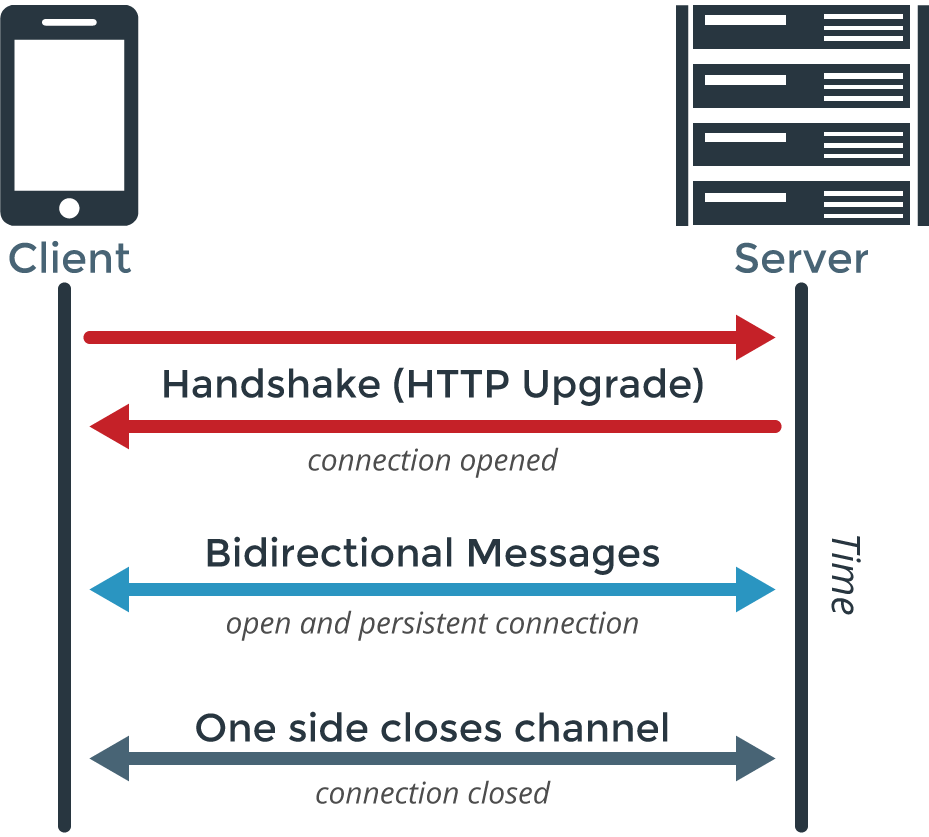
\includegraphics[width=0.6\textwidth, keepaspectratio=true]{websockets-diagram}
	\centering
	\caption[Diagrama de conexão via websocket]{Diagrama de conexão via websocket}
	\fonte{\url{https://www.pubnub.com/learn/glossary/what-is-websocket/}{}}
	\label{fig:websocket-diagram}
\end{figure}
\FloatBarrier


\subsection[\textit{SQL}]{\textit{SQL}}\label{sql}
A linguagem teve seu início dentro de um projeto chamado \textit{System R} que pertencia a IBM em meados dos anos 70. Structured Query Language, ou
comumente conhecida como SQL é uma linguagem padrão de banco de dados, se tornou bastante conhecida e usada devido a sua simplicidade e facilidade 
de uso. Diferentemente das outras linguagens de banco de dados a consulta em SQL especifica a forma do resultado e não o caminho para chegar nele, uma outra
grande diferena é que a linguagem SQL é declarativa diferindo mais uma vez das outras linguagens que por sua vez são procedurais.

O MySQL é um sistema de gerenciamento de banco de dados que utiliza a linguagem SQL. Atualmente é o sistema mais popular em gerenciamento de 
banco de dados. Sua rápida popularização deve-se a fácil comuniação entre servidor e aplicação. 

\begin{figure}[h!]
	
\includegraphics[width=0.5\textwidth, keepaspectratio=true]{mysql}
	\centering
	\caption[MySQL]{MySql}
	\fonte{\url{https://www.infoescola.com/wp-content/uploads/2011/01/mysql.jpg}{}}
	\label{fig:mysql-image}
\end{figure}
\FloatBarrier

\subsection[\textit{Fritzing}]{\textit{Fritzing}}\label{fritzing}
O \textit{Fritzing} é uma iniciativa \textit{open source} que inicialmente foi
designada a desenvolvedores amadores que gostasse de tirar a sua ideia do papel. Em poucas palavras
a plataforma auxilia os desenvolvedores por meio de uma interface gráfica nas primeiras montagens com Arduino
ou outro microcontrolador, sua intuitiva interface proporciona ao usuário uma rápida montagem do circuito em protoboard. O \textit{software} vai além
e permite com que os desenvolvedores tenha uma visão tanto da protoboar, como do esquemático elétrico. 


\section[\textit{Componentes Físicos}]{\textit{Componentes Físicos}}\label{comp-fisico}
No decorrer do desenvolvimento do hardwaare fez-se uso de alguns componentes eletrônicos, microcontrolador que serão descritos nessa seção.
\subsection[\textit{ESP8266}]{\textit{ESP8266}}\label{esp}
É um microcontrolador que é produzido por um fabricante chinês - Espressif - que tem como principal vantagem a comunicação \textit{Wi-Fi} já integrada em seu circuito.
O chip teve seu auge em 2014 quando "estourou" na cultura \textit{maker} com o ESP-01, essa placa permite que microcontroladores se conectem a uma rede
sem fio  fazendo conexões TCP/IP, tendo a capacidade de ser servidor ou cliente.

\begin{figure}[h!]
	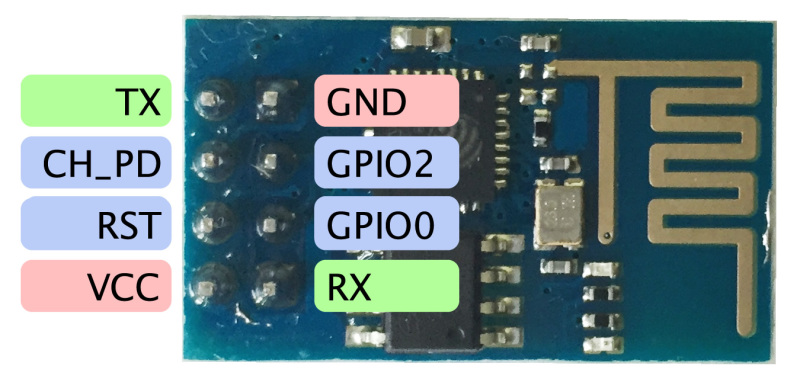
\includegraphics[width=0.3\textwidth, keepaspectratio=true]{esp8266}
	\centering
	\caption[ESP8266]{ESP8266}
	\fonte{\url{http://fabacademy.org/archives/2015/doc/images/esp-01.jpg}{}}
	\label{fig:esp8266}
\end{figure}
\FloatBarrier

O NodeMcu é uma plataforma \textit{IoT} totalmente \textit{open source}. Tem como principal linguagem de script Lua, foi construído sobre o SDK ESP8266.
A plataforma surgiu pouco tempo após o lançamento do ESP8266 (\autoref{esp}). A plataforma logo conquistou o seu espaço, pois trazia um conjunto
de circuitos já previamente embutido que o ESP8266 por si só não proporcionava.

\begin{figure}[h!]
	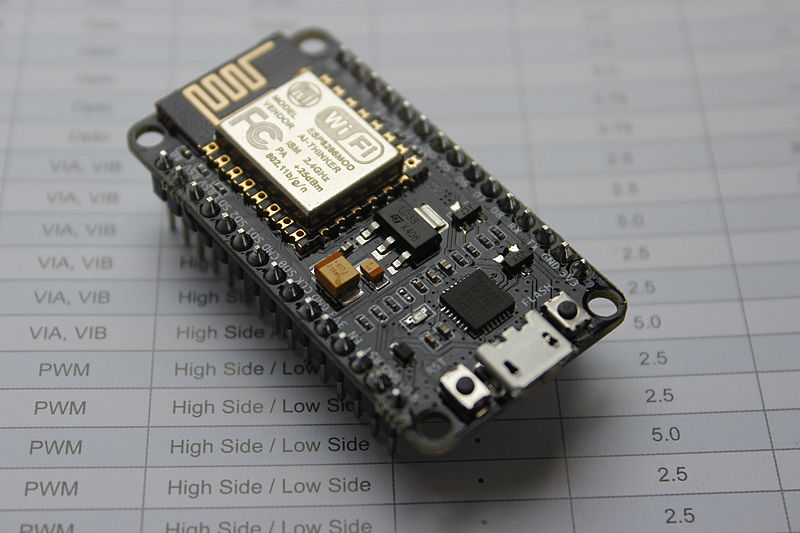
\includegraphics[width=0.6\textwidth, keepaspectratio=true]{nodemcu}
	\centering
	\caption[NodeMCU]{NodeMCU}
	\fonte{\url{https://upload.wikimedia.org/wikipedia/commons/7/7e/NodeMCU_DEVKIT_1.0.jpg}{}}
	\label{fig:nodemcu}
\end{figure}
\FloatBarrier

\subsection[\textit{Sensor de Corrente SCT 013-000}]{\textit{Sensor de Corrente SCT 013-000}}\label{sct}
O Sensor é um ótimo transformador de corrente para leituras não invasivas, possuindo um fucionamento bem similar a de um alicate amperímetro. Com a seguinte especificação
técnica: 
\begin{itemize}
	\item 100A no primário
	\item saída de 50mA no secundário
	\item Temperatura máxima \ang{70}C
	\item Temperatura mínima \ang{-25}C
\end{itemize} 
Para realizar a leitura da corrente sem a necessidade de contato elétrico o sensor de corrente alternada utiliza as propriedades 
magnéticas da corrente elétrica. O SCT é um sensor do tipo Transformador de Corrente, que resumidamente nada mais é que um conjunto de espiras que são
colocadas ao redor do condutor ao qual se quer medir a corrente 

\begin{figure}[h!]
	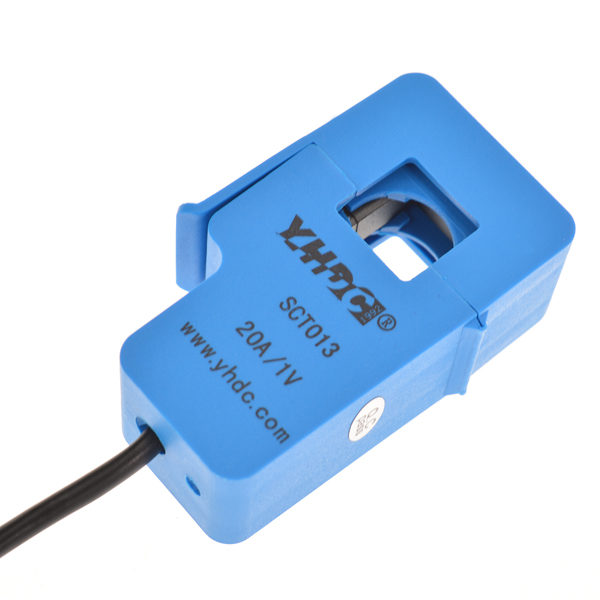
\includegraphics[width=0.4\textwidth, keepaspectratio=true]{sct}
	\centering
	\caption[SCT-013-000]{SCT-013-000}
	\fonte{\url{https://uploads.filipeflop.com/2017/07/1-34.jpg}{}}
	\label{fig:sct}
\end{figure}
\FloatBarrier
